%%%%%%%%%%%%%%%%%%%%%%%%%%%%%%%%%%%%%%%%%
% Short Sectioned Assignment LaTeX Template Version 1.0 (5/5/12)
% This template has been downloaded from: http://www.LaTeXTemplates.com
% Original author:  Frits Wenneker (http://www.howtotex.com)
% License: CC BY-NC-SA 3.0 (http://creativecommons.org/licenses/by-nc-sa/3.0/)
%%%%%%%%%%%%%%%%%%%%%%%%%%%%%%%%%%%%%%%%%

%----------------------------------------------------------------------------------------
%	PACKAGES AND OTHER DOCUMENT CONFIGURATIONS
%----------------------------------------------------------------------------------------

\documentclass[paper=a4, fontsize=11pt]{scrartcl} % A4 paper and 11pt font size

% ---- Entrada y salida de texto -----

\usepackage[T1]{fontenc} % Use 8-bit encoding that has 256 glyphs
\usepackage[utf8]{inputenc}
%\usepackage{fourier} % Use the Adobe Utopia font for the document - comment this line to return to the LaTeX default

% ---- Idioma --------

\usepackage[spanish, es-tabla]{babel} % Selecciona el español para palabras introducidas automáticamente, p.ej. "septiembre" en la fecha y especifica que se use la palabra Tabla en vez de Cuadro

% ---- Otros paquetes ----
\usepackage{alltt}
\usepackage{hyperref}
\usepackage{url} % ,href} %para incluir URLs e hipervínculos dentro del texto (aunque hay que instalar href)
\usepackage{amsmath,amsfonts,amsthm} % Math packages
%\usepackage{graphics,graphicx, floatrow} %para incluir imágenes y notas en las imágenes
\usepackage{graphics,graphicx, float} %para incluir imágenes y colocarlas

\usepackage{cite}
\usepackage{listings}
\usepackage{xcolor}

% Para hacer tablas comlejas
%\usepackage{multirow}
%\usepackage{threeparttable}

%\usepackage{sectsty} % Allows customizing section commands
%\allsectionsfont{\centering \normalfont\scshape} % Make all sections centered, the default font and small caps

\usepackage{fancyhdr} % Custom headers and footers

\setcounter{secnumdepth}{0}
\pagestyle{fancyplain} % Makes all pages in the document conform to the custom headers and footers
\fancyhead{} % No page header - if you want one, create it in the same way as the footers below
\fancyfoot[L]{} % Empty left footer
\fancyfoot[C]{} % Empty center footer
\fancyfoot[R]{\thepage} % Page numbering for right footer
\renewcommand{\headrulewidth}{0pt} % Remove header underlines
\renewcommand{\footrulewidth}{0pt} % Remove footer underlines
\setlength{\headheight}{13.6pt} % Customize the height of the header

\numberwithin{equation}{section} % Number equations within sections (i.e. 1.1, 1.2, 2.1, 2.2 instead of 1, 2, 3, 4)
\numberwithin{figure}{section} % Number figures within sections (i.e. 1.1, 1.2, 2.1, 2.2 instead of 1, 2, 3, 4)
\numberwithin{table}{section} % Number tables within sections (i.e. 1.1, 1.2, 2.1, 2.2 instead of 1, 2, 3, 4)

\setlength\parindent{0pt} % Removes all indentation from paragraphs - comment this line for an assignment with lots of text

\newcommand{\horrule}[1]{\rule{\linewidth}{#1}} % Create horizontal rule command with 1 argument of height


%----------------------------------------------------------------------------------------
%	TÍTULO Y DATOS DEL ALUMNO
%----------------------------------------------------------------------------------------

\title{	
\normalfont \normalsize 
\textsc{\textbf{Ingeniería de Servidores (2016-2017)} \\ Grado en Ingeniería Informática \\ Universidad de Granada} \\ [25pt] % Your university, school and/or department name(s)
\horrule{0.5pt} \\[0.4cm] % Thin top horizontal rule
\huge Memoria Práctica 4 \\ % The assignment title
\horrule{2pt} \\[0.5cm] % Thick bottom horizontal rule
}

\author{José Álvaro Garrido López} % Nombre y apellidos

\date{\normalsize\today} % Incluye la fecha actual

%----------------------------------------------------------------------------------------
% DOCUMENTO
%----------------------------------------------------------------------------------------

\begin{document}
\maketitle % Muestra el Títuolo

\newpage %inserta un salto doe página

\tableofcontents % para generar el índice de contenidos

\listoffigures

\newpage

\newpage

\section{Cuestión 1. Seleccione, instale y ejecute uno, comente los resultados. \textbf{Atención:} no es lo mismo un benchmark que una suite, instale un benchmark.}

Según la documentación proporcionada en \cite{phoronix}, con el comando
\begin{verbatim}
phoronix-test-suite list-available-tests
\end{verbatim}
podemos listar todos los tests disponibles para ejecutar en una máquina, así como se observa en \ref{cuestion1-01}.
En la primera columna aparece el \textit{id} del test, que se utilizará para instalarlo o ejecutarlo, en la del medio el \textit{nombre} (más descriptivo) del test, y en la tercera columna el componente \textit{hardware} que se va a evaluar.

\begin{figure}[H]
	\centering
	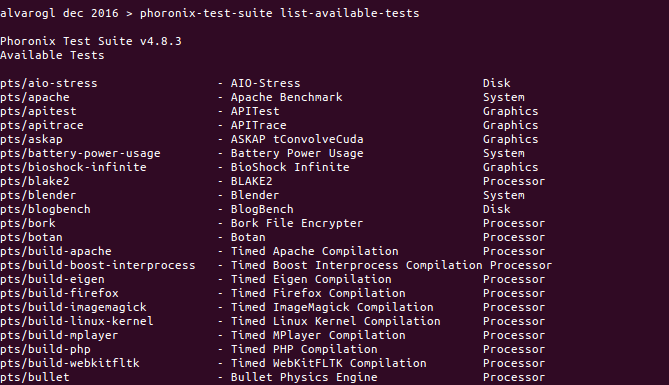
\includegraphics[scale=0.6]{cuestion1-01.png}
	\caption{Listado de los tests disponibles de \textit{phoronix}} \label{cuestion1-01}
\end{figure}

En mi caso, he escogido el test de \textit{aio-stress}, que consiste en un \textit{benchmark} de E/S (entrada/salida) aleatoria asíncrona, este test sirve para evaluar las prestaciones de la unidad de almacenamiento del equipo sobre el que se ejecute. Se puede encontrar en \cite{aio-stress}.

Como se observa en \ref{cuestion1-02}, para instalar el \textit{benchmark} mencionado, simplemente ejecutamos:

\begin{verbatim}
phoronix-test-suite install <id-test>
\end{verbatim}

\begin{figure}[H]
	\centering
	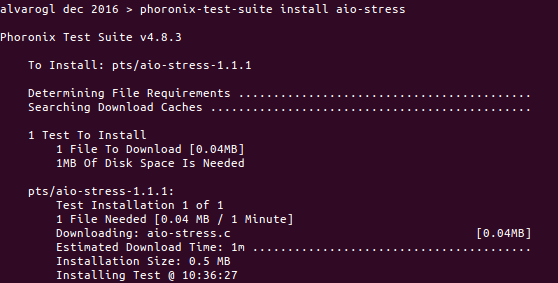
\includegraphics[scale=0.6]{cuestion1-02.png}
	\caption{Instalación del \textit{benchmark: aio-stress}} \label{cuestion1-02}
\end{figure}

Una vez instalado, para ejecutarlo la sintaxis es la siguiente:

\begin{verbatim}
phoronix-test-suite run <id-test>
\end{verbatim}

En \ref{cuestion1-03} y en \ref{cuestion1-04} se presenta una ejecución del \textit{benchmark}.

En \ref{cuestion1-03} se muestra información reconocida por el \textit{benchmark} sobre el \textit{hardware} del equipo, y sobre el sistema operativo, el sistema de archivos, la versión del \textit{kernel} y del entorno gráfico. También se especifican las anteriores ejecuciones del test, y nos pregunta por el nombre que le queremos dar a esta nueva ejecución (importante para consultarla posteriormente).

\begin{figure}[H]
	\centering
	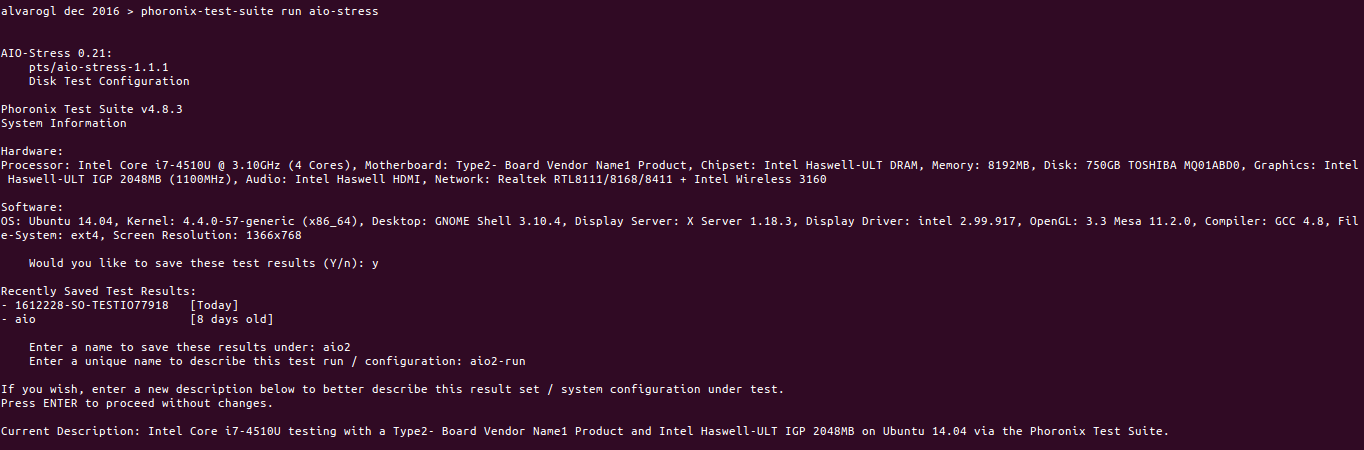
\includegraphics[scale=0.35]{cuestion1-03.png}
	\caption{Ejecución de \textit{aio-stress}} \label{cuestion1-03}
\end{figure}

En \ref{cuestion1-04} salen los resultados del test ejecutado.
Se realizan tres intentos y se hace la media, en este caso el resultado es de 76.73 MB/s. Esto significa que nuestra unidad de almacenamiento, en este sistema y en estas condiciones, es capaz de escribir datos en pistas aleatorias del disco a una velocidad de 76.73 MB/s.

\begin{figure}[H]
	\centering
	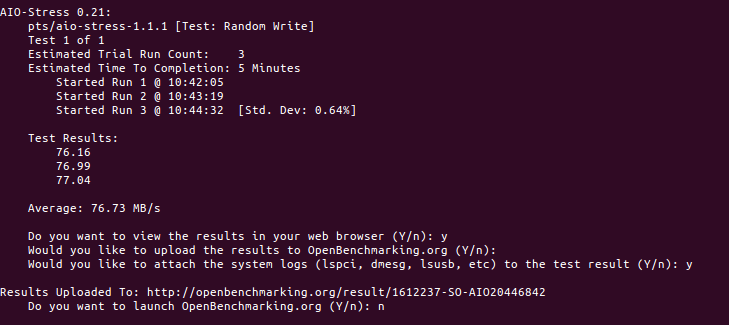
\includegraphics[scale=0.6]{cuestion1-04.png}
	\caption{Ejecución de \textit{aio-stress}. Resultados} \label{cuestion1-04}
\end{figure}


\textit{Phoronix} almacena un archivo en \textit{/home/<usuario>/.phoronix-test-suite/test-results/<nombre-ejecucion-test>/composite.xml} en el que se puede consultar la información recabada por el \textit{benchmark} acompañada de algunas tablas y gráficos como se muestra en \ref{cuestion1-05} y en \ref{cuestion1-06}. Dicho archivo se abre con un navegador y se puede acceder desde la línea de comandos mediante:

\begin{verbatim}
phoronix-test-suite show-result <nombre-ejecucion-test>
\end{verbatim}

Como en mi caso grabé la ejecución del test con el nombre \textit{aio2}, tuve que ejecutar:

\begin{verbatim}
phoronix-test-suite show-result aio2
\end{verbatim}

\begin{figure}[H]
	\centering
	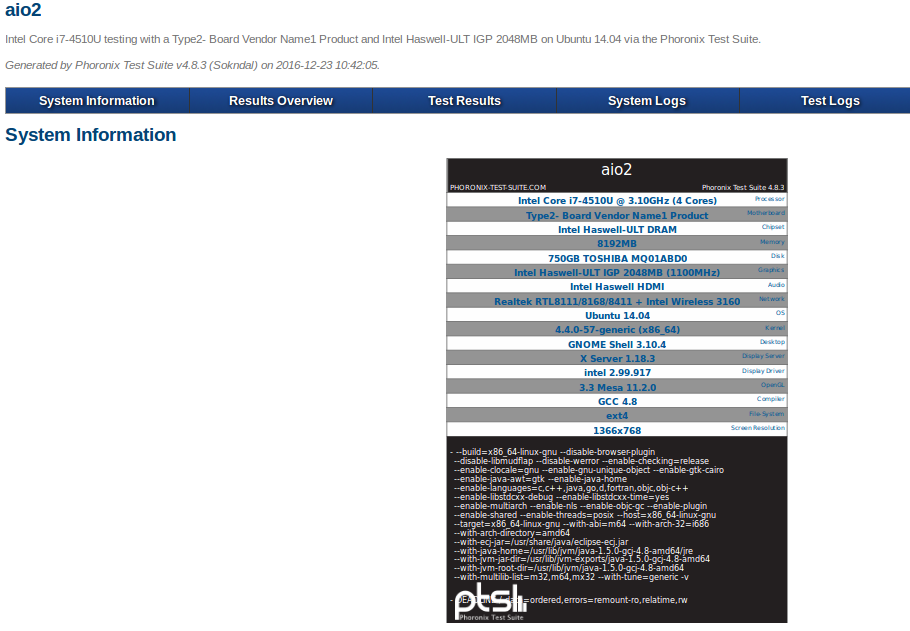
\includegraphics[scale=0.45]{cuestion1-05.png}
	\caption{Resultados de la ejecución del test} \label{cuestion1-05}
\end{figure}

\begin{figure}[H]
	\centering
	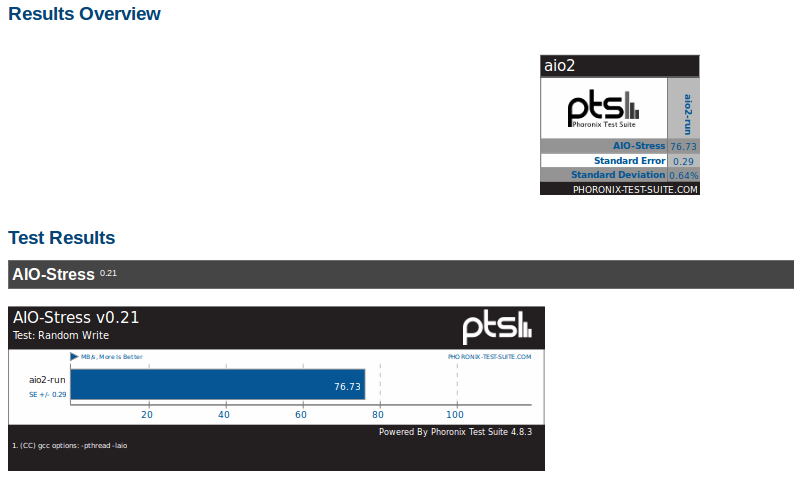
\includegraphics[scale=0.5]{cuestion1-06.png}
	\caption{Resultados de la ejecución del test} \label{cuestion1-06}
\end{figure}

Una de las características que me han parecido interesantes de \textit{Phoronix} es la de poder comparar tus ejecuciones de \textit{benchmark} con las de los demás.
En \cite{aio-stress}, aparece una lista con las ejecuciones más recientes del test, como se muestra en \ref{cuestion1-07}.

\begin{figure}[H]
	\centering
	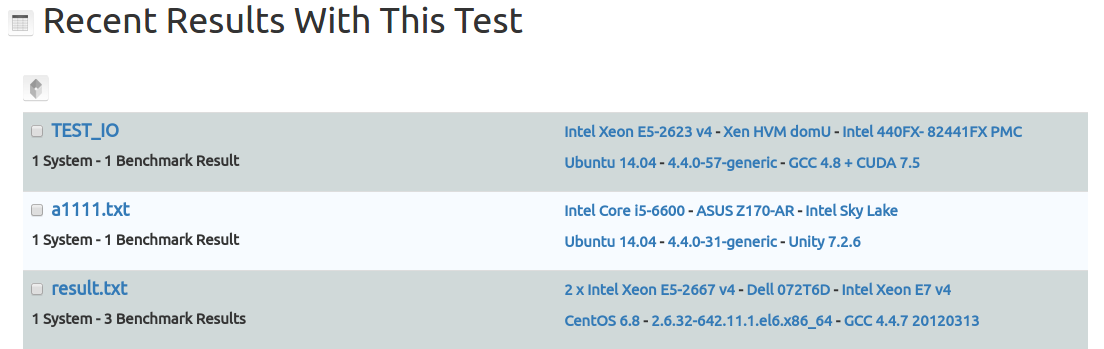
\includegraphics[scale=0.45]{cuestion1-07.png}
	\caption{Resultados recientes del test} \label{cuestion1-07}
\end{figure}

En mi caso he elegido un test ejecutado en un equipo con procesador Intel Xeon E5-2623 v4, de 8 \textit{cores} a 2.60 Ghz, y una unidad de almacenamiento de 48 GB, de la que no se ofrecen especificaciones.

Los resultados se pueden ver en \ref{cuestion1-08}.

\begin{figure}[H]
	\centering
	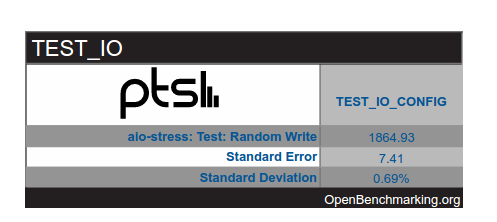
\includegraphics[scale=0.6]{cuestion1-08.png}
	\caption{Resultados del test con Intel Xeon E5} \label{cuestion1-08}
\end{figure}

En la propia página del resultado de este test, se describe cómo realizar la comparativa con dicha ejecución \ref{cuestion1-09}.

\begin{figure}[H]
	\centering
	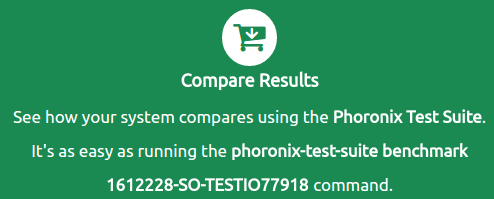
\includegraphics[scale=0.4]{cuestion1-09.png}
	\caption{Instrucciones para comparar ejecuciones del \textit{benchmark}} \label{cuestion1-09}
\end{figure}

Al ejecutar esa línea de comandos, se realiza una nueva ejecución del test, y al final se nos pregunta si deseamos abrir el navegador para ver la comparación, tal y como se muestra en \ref{cuestion1-10} y en \ref{cuestion1-11}.

\begin{figure}[H]
	\centering
	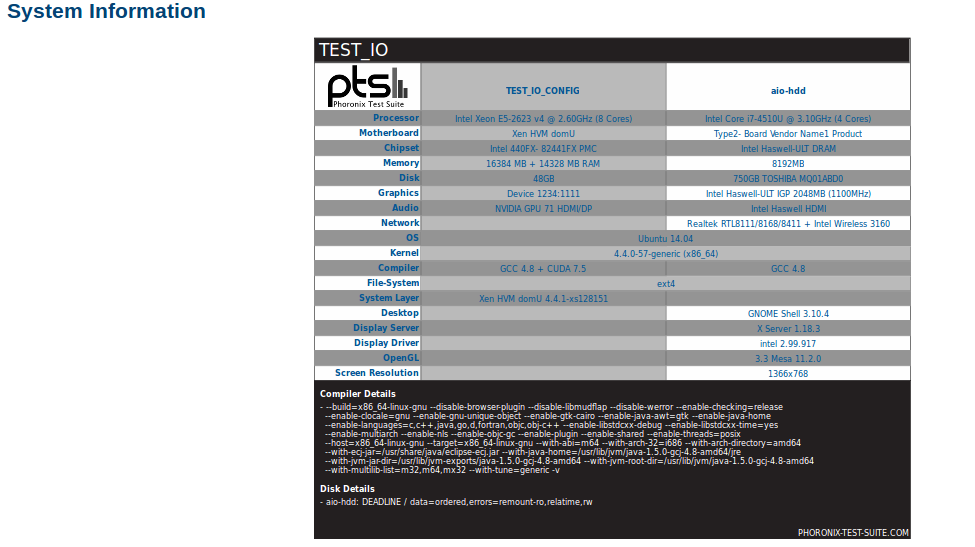
\includegraphics[scale=0.5]{cuestion1-10.png}
	\caption{Comparación del \textit{hardware}} \label{cuestion1-10}
\end{figure}

\begin{figure}[H]
	\centering
	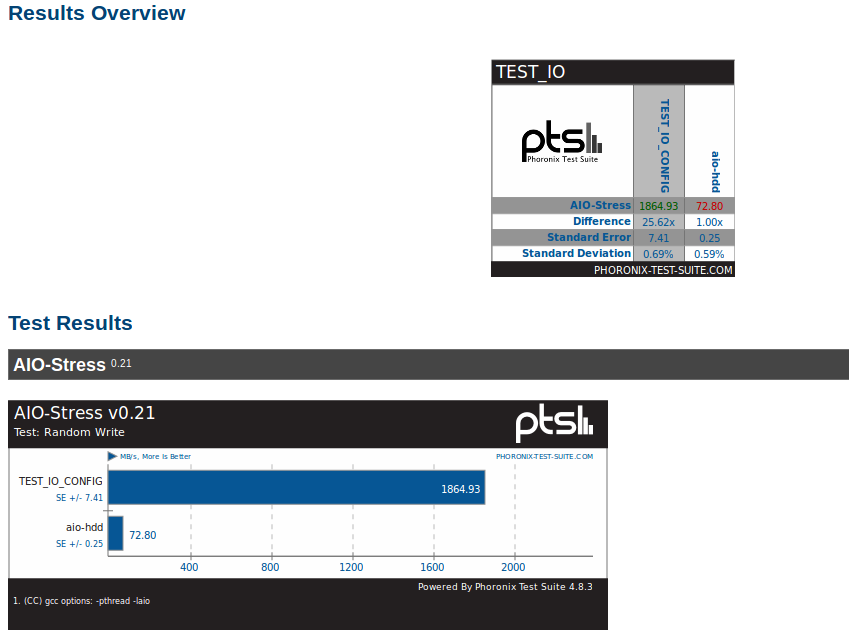
\includegraphics[scale=0.4]{cuestion1-11.png}
	\caption{Resultados de la comparación} \label{cuestion1-11}
\end{figure}

Como se ve en \ref{cuestion1-11}, el otro equipo ha sido un 25.62 mejor en el test, llegando a escribir en disco a una velocidad de 1864.93 MB/s. Se deduce, por la potencia del procesador y el rendimiento del disco, que se trata de un computador de altas prestaciones, aunque con muy poca capacidad de disco.

Se pueden exportar los resultados de la ejecución de un test o los de una comparación a un archivo .csv o .pdf si ejecutamos:

\begin{verbatim}
phoronix-suite-test result-export-to-<formato> <nombre-ejecucion-test>
\end{verbatim}

La comparación será adjuntada al archivo comprimido de la entrega como \url{1612228-SO-TESTIO77918.csv}.
\newline
\newline
Nota: Cada vez que se alude a expresiones como \textit{escribir en disco} o \textit{rendimiento del disco}, las mismas se refieren a la unidad de almacenamiento  del equipo en cuestión, sea esta un SSD (Solid State Drive), un HDD (Hard Disk Drive) o cualquier otra.

\section{Cuestión 2. De los parámetros que le podemos pasar al comando, ¿qué significa -c 5? ¿y -n 100? Monitorice la ejecución de ab contra alguna máquina (cualquiera). ¿Cuántas $"$tareas$"$ crea ab en el cliente?}

Según \cite{ab}, la opción -c se refiere a la concurrencia, en concreto al número de peticiones múltiples a realizar simultáneamente. El valor por defecto es de una petición a la vez. Por lo que -c 5 significa que \textit{ab} realizará 5 peticiones a la vez.

La opción -n sirve para determinar el número de veces que se van a realizar las peticiones para la sesión de \textit{benchmarking}. El parámetro -n 100 realizará las peticiones 100 veces. Como se explica en la documentación, el valor por defecto es de uno, pero es demasiado pequeño como para que las consecuencias sean notorias (como normalmente se pretende en un \textit{benchmark}), así que será necesario para nuestro caso aumentar este valor.

Debemos tener en cuenta, que para acceder desde la máquina anfitriona a la virtual, necesitamos una interfaz de red que haga visible la virtual desde la anfitriona, por ejemplo, la red solo-anfitrión, como se explica en \cite{redvb} y en anteriores prácticas \ref{cuestion2-01}.

\begin{figure}[H]
	\centering
	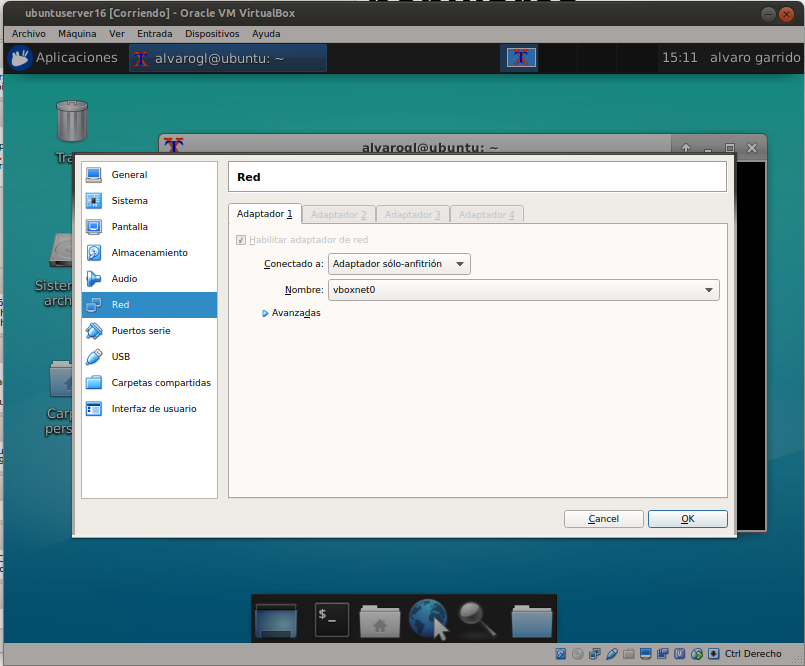
\includegraphics[scale=0.6]{cuestion2-01.png}
	\caption{Tipo de red para la máquina virtual} \label{cuestion2-01}
\end{figure}

Es posible cambiar la interfaz de red con la máquina encendida, en este caso, puede ocurrir que después de esto necesitemos reiniciar los servicios de red, para que el sistema tome la nueva IP con la interfaz virtual de la red actualizada. Esto, como se explica en \cite{network}, se puede conseguir ejecutando en terminal:

\begin{verbatim}
sudo /etc/init.d/networking restart
\end{verbatim}

Observamos con la orden \textit{top} los procesos que hay activos en la máquina virtual como se ve en la imagen \ref{cuestion2-02}

\begin{figure}[H]
	\centering
	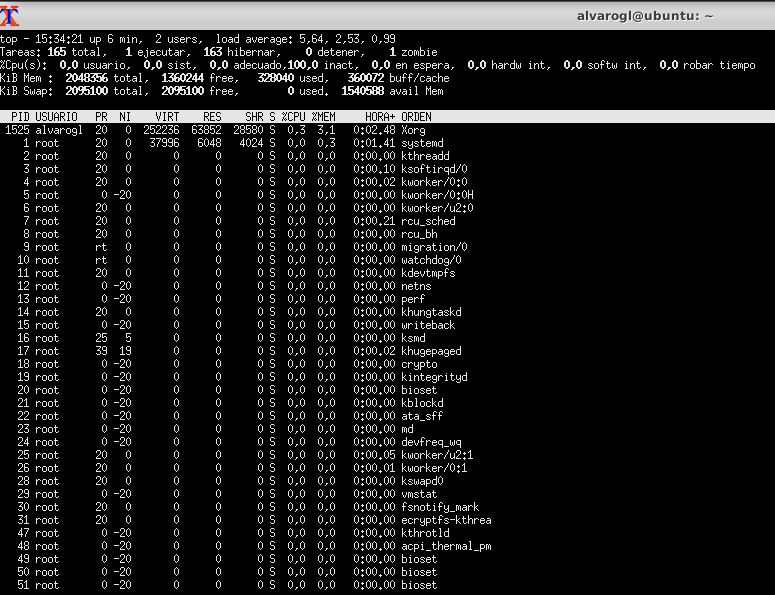
\includegraphics[scale=0.35]{cuestion2-02.png}
	\caption{Procesos activos de la máquina virtual antes de lanzar las peticiones} \label{cuestion2-02}
\end{figure}

Ejecutamos:

\begin{verbatim}
ab -c 5 -n 1000 http://<ip>/
\end{verbatim}

En este caso, la IP de la máquina virtual, como se muestra en \ref{cuestion2-07}, es 192.168.56.103.

\begin{figure}[H]
	\centering
	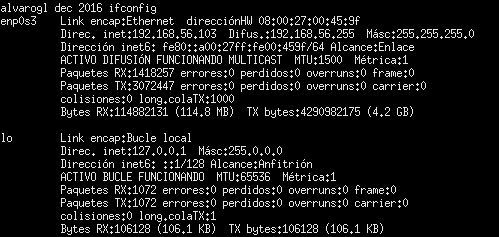
\includegraphics[scale=0.6]{cuestion2-07.png}
	\caption{IP de la máquina virtual con Ubuntu Server} \label{cuestion2-07}
\end{figure}

Si ejecutamos 100 como se describe en el enunciado, da poco tiempo a ver los nuevos procesos con \textit{top}. El resultado de esta ejecución se puede ver en \ref{cuestion2-04} y \ref{cuestion2-05}.

\begin{figure}[H]
	\centering
	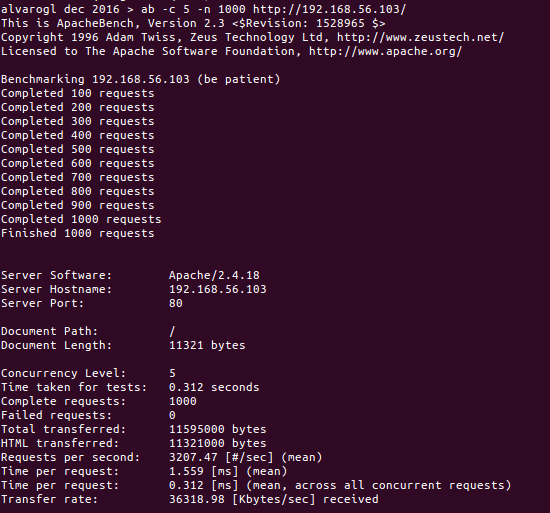
\includegraphics[scale=0.5]{cuestion2-04.png}
	\caption{Resultado de la ejecución de ab contra la máquina virtual} \label{cuestion2-04}
\end{figure}

\begin{figure}[H]
	\centering
	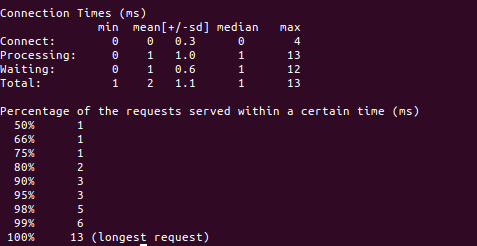
\includegraphics[scale=0.5]{cuestion2-05.png}
	\caption{Resultado de la ejecución de ab contra la máquina virtual} \label{cuestion2-05}
\end{figure}

Se han tardado 0.312 segundos en realizar todas las peticiones.
Mientras se lanzan las peticiones, \textit{top} nos muestra que se han creado 10 procesos nuevos de \textit{apache2} en el cliente, como se puede ver en \ref{cuestion2-03}.

\begin{figure}[H]
	\centering
	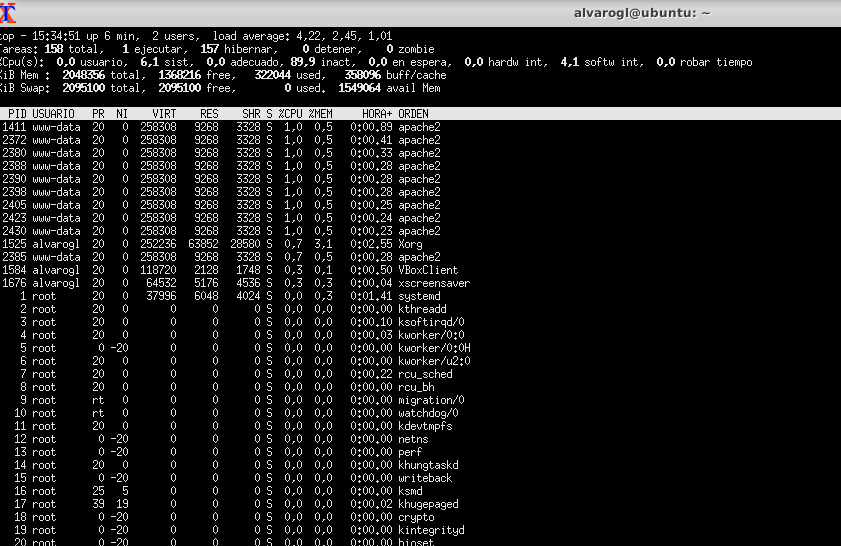
\includegraphics[scale=0.45]{cuestion2-03.png}
	\caption{Orden \textit{top}. Creación de nuevos procesos de \textit{apache2} en el cliente} \label{cuestion2-03}
\end{figure}

En el \textit{host} se crea un proceso, \textit{ab} \ref{cuestion2-06}

\begin{figure}[H]
	\centering
	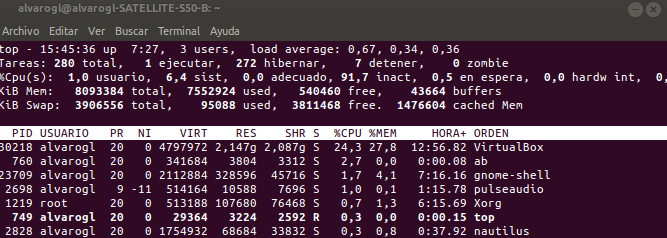
\includegraphics[scale=0.6]{cuestion2-06.png}
	\caption{Creación de un proceso en el \textit{host}} \label{cuestion2-06}
\end{figure}

\section{Cuestión 3. Ejecute ab contra las tres máquinas virtuales (desde el SO anfitrión a las máquinas virtuales de la red local). ¿Cuál es la que proporciona mejores resultados? Muestre y coméntelos. (Use como máquina de referencia Ubuntu Server para la comparativa).}

Para esta cuestión, como se expone en el enunciado, tomaremos como referencia la máquina de Ubuntu Server. Los resultados de la prueba realizada contra esta máquina se muestran en \ref{cuestion2-04} y en \ref{cuestion2-05}.

Se realizaron un total de 1000 peticiones, las cuales tardaron un total de 0.312 segundos en finalizar. El tiempo por petición fue de 0.312 milisegundos (teniendo en cuenta la concurrencia de peticiones). Se transmitieron en total 11595000 bytes, a una velocidad de 36318.98 KB/s.
El 99\% de las peticiones se sirvieron en 6 ms o menos cada una, el 100\% en 13 ms o menos.

En cuanto a CentOS, los resultados del \textit{benchmark} son los que se describen en \ref{cuestion3-02} y en \ref{cuestion3-03}.
La IP de la máquina es 192.168.56.102 \ref{cuestion3-01}.

\begin{figure}[H]
	\centering
	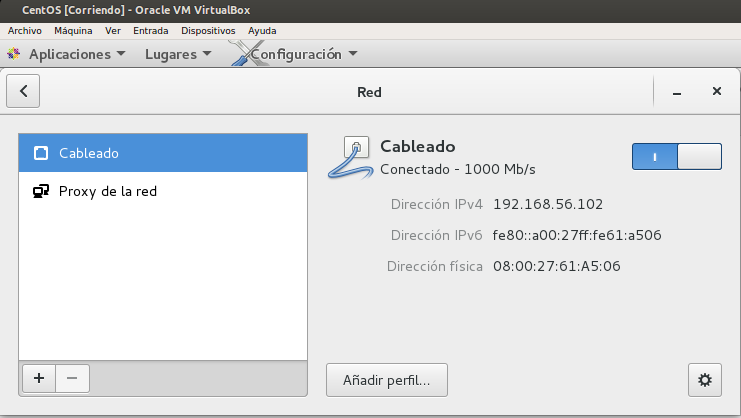
\includegraphics[scale=0.6]{cuestion3-01.png}
	\caption{IP de la máquina virtual con CentOS} \label{cuestion3-01}
\end{figure}

\begin{figure}[H]
	\centering
	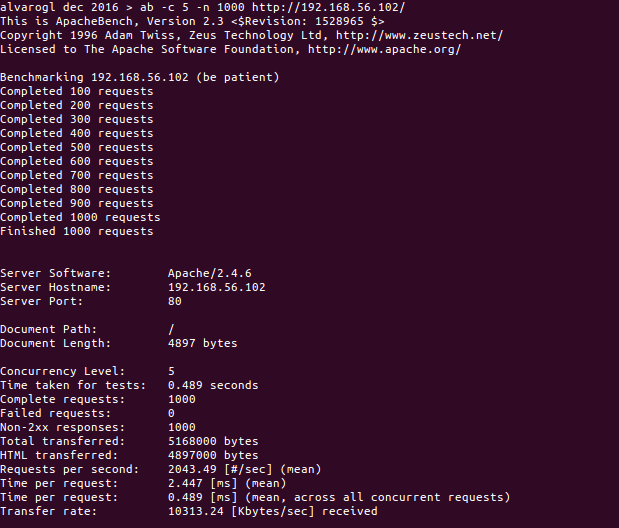
\includegraphics[scale=0.6]{cuestion3-02.png}
	\caption{Resultados del \textit{benchmark} con CentOS} \label{cuestion3-02}
\end{figure}

\begin{figure}[H]
	\centering
	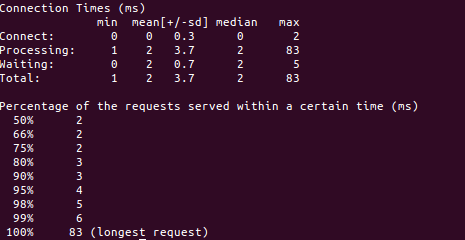
\includegraphics[scale=0.6]{cuestion3-03.png}
	\caption{Resultados del \textit{benchmark} con CentOS} \label{cuestion3-03}
\end{figure}

En este caso, se realizaron 1000 peticiones en 0.489 segundos, un 50 \% más lento que en Ubuntu, un total de 5168000 bytes (la mitad que en Ubuntu), y el tiempo por petición fue de 0.489 milisegundos, a 10313.24 KB/s. El 99\% de las peticiones se sirvieron en 6 ms o menos, el 100\% en 83 ms.
Parece que en CentOS hay un 1\% de peticiones que se sirven mucho más lentas (puede ser porque se realiza algún tipo de comprobación al terminar de servir todas las peticiones).

En Windows, cuya IP se muestra en \ref{cuestion3-04}, y resultados del \textit{benchmark} en \ref{cuestion3-05} y \ref{cuestion3-06}, el tiempo de servicio total de las peticiones ha sido de 0.269 segundos, a 0.269 ms cada petición (velocidad de 925.83 KB/s), el número de bytes transferidos es de 255000, muchos menos bytes que en los resultados de los otros dos sistemas operativos, pero más rápido el servicio de las peticiones. El 100\% de las peticiones se sirvieron en 5 ms o menos cada una, tiempo que supera a CentOS y Ubuntu Server (Windows 15\% mejor en esto), siendo Windows el más rápido en servirlas.

\begin{figure}[H]
	\centering
	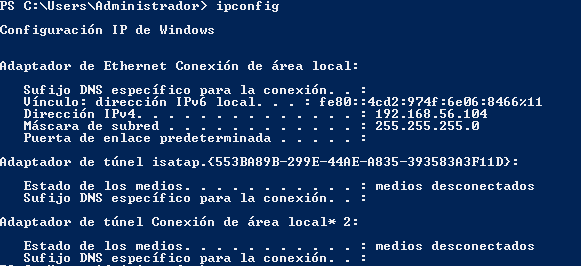
\includegraphics[scale=0.6]{cuestion3-04.png}
	\caption{IP de Windows Server 2008 R2} \label{cuestion3-04}
\end{figure}

\begin{figure}[H]
	\centering
	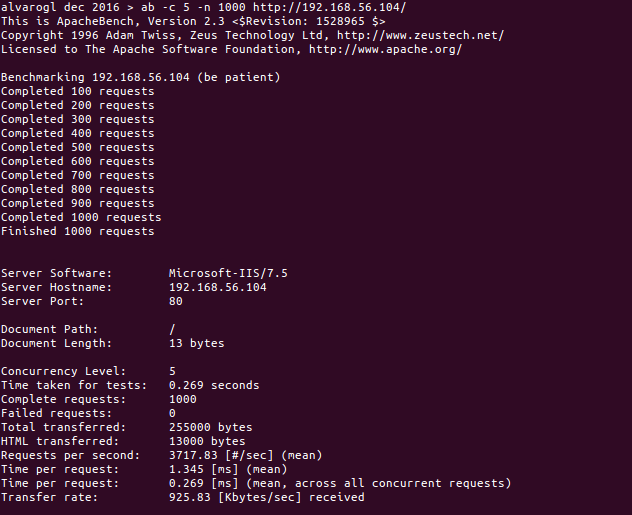
\includegraphics[scale=0.6]{cuestion3-05.png}
	\caption{Resultados del \textit{benchmark} sobre Windows Server} \label{cuestion3-05}
\end{figure}

\begin{figure}[H]
	\centering
	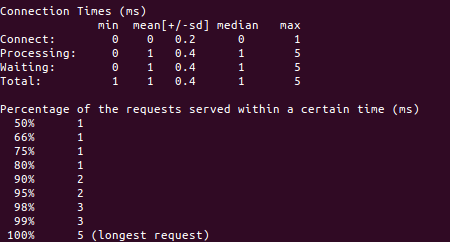
\includegraphics[scale=0.6]{cuestion3-06.png}
	\caption{Resultados del \textit{benchmark} sobre Windows Server} \label{cuestion3-06}
\end{figure}

En \ref{cuestion3-07} se muestra la comparativa de las tres ejecuciones.

\begin{figure}[H]
	\centering
	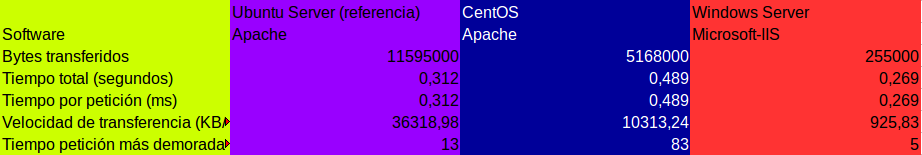
\includegraphics[scale=0.45]{cuestion3-07.png}
	\caption{Comparativa de las ejecuciones (fuente propia)} \label{cuestion3-07}
\end{figure}

\section{Cuestión 4. Instale y siga el tutorial en http://jmeter.apache.org/usermanual/build-web-test-plan.html realizando capturas de pantalla y comentándolas. En vez de usar la web de jmeter, haga el experimento usando sus máquinas virtuales, ¿coincide con los resultados de ab?}

Según el tutorial de \cite{jmeter}, primero debemos crear el grupo de hilos (grupo de usuarios), como se muestra en \ref{cuestion4-01} con 5 usuarios, periodo de subida 1 y contador del bucle 2.

\begin{figure}[H]
	\centering
	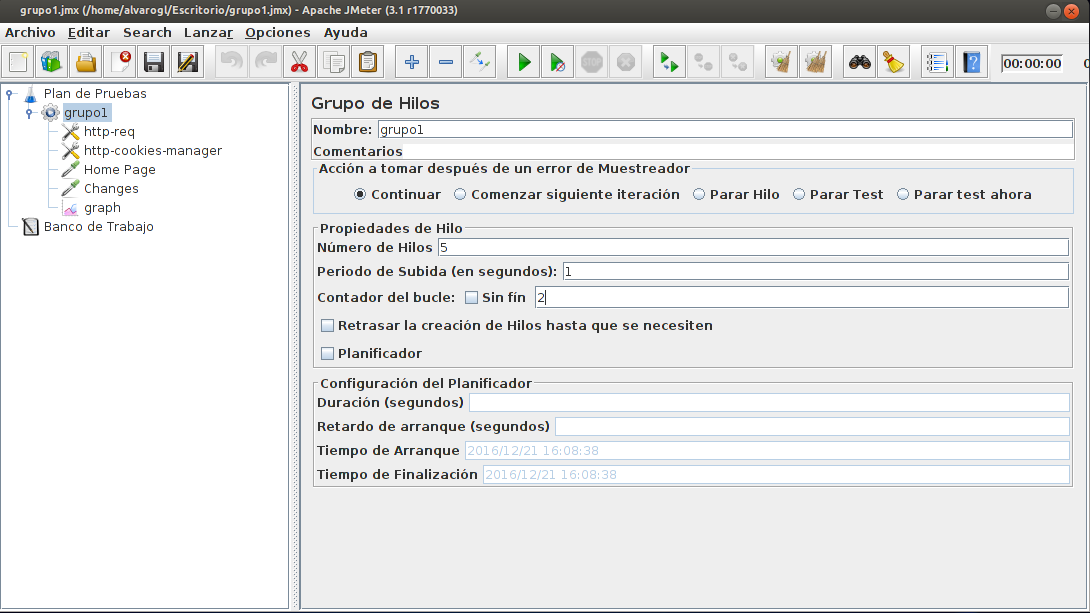
\includegraphics[scale=0.4]{cuestion4-01.png}
	\caption{Crear grupo de hilos (usuarios)} \label{cuestion4-01}
\end{figure}

Creamos un nuevo elemento para determinar los valores por defecto de las peticiones HTTP. En mi caso las pruebas se realizarán primero contra la IP de mi máquina virtual con Ubuntu Server \ref{cuestion4-02}.

\begin{figure}[H]
	\centering
	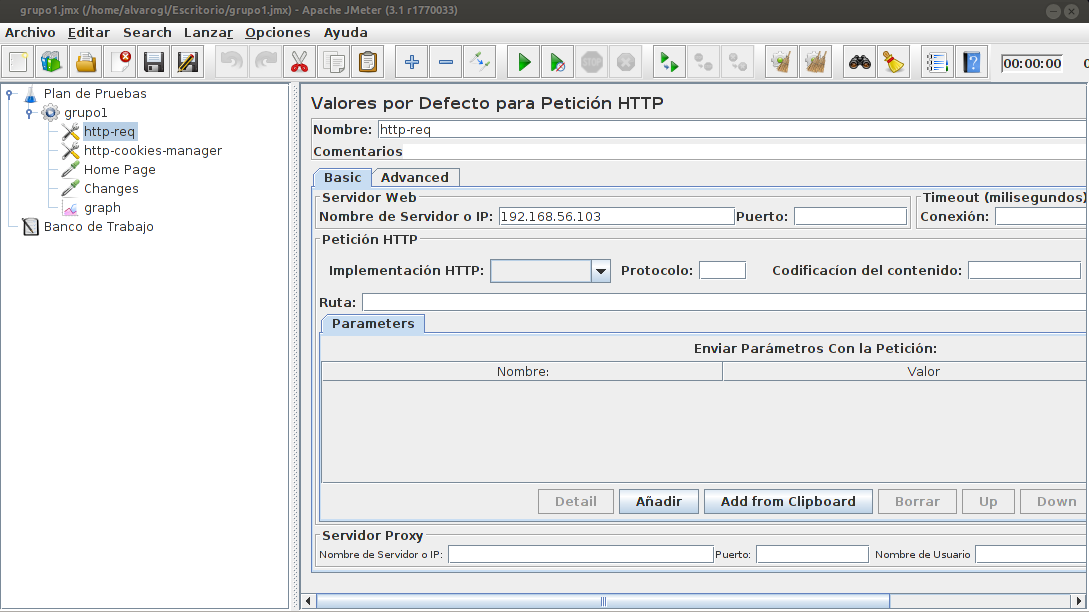
\includegraphics[scale=0.4]{cuestion4-02.png}
	\caption{Configuración de las peticiones} \label{cuestion4-02}
\end{figure}

Creamos un manejador de \textit{cookies}, para que cada hebra tenga sus propias \textit{cookies}, como se explica en \cite{jmeter}. Ver \ref{cuestion4-03}

\begin{figure}[H]
	\centering
	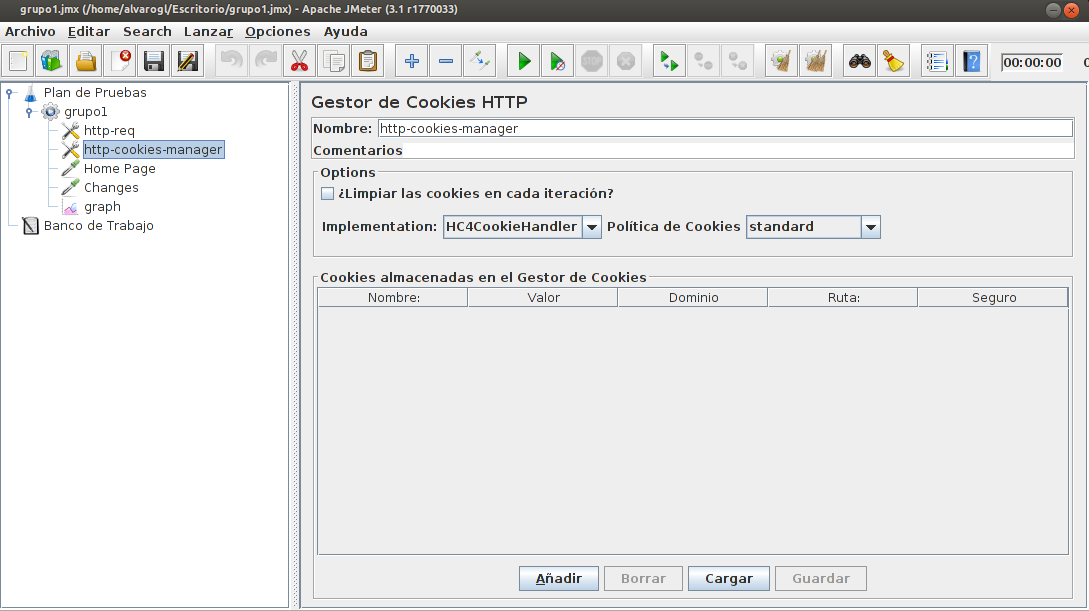
\includegraphics[scale=0.4]{cuestion4-03.png}
	\caption{Configuración del manejador de \textit{cookies}} \label{cuestion4-03}
\end{figure}

Seleccionamos el nombre y la ruta de las peticiones HTTP, como se indica en \ref{cuestion4-04}.

\begin{figure}[H]
	\centering
	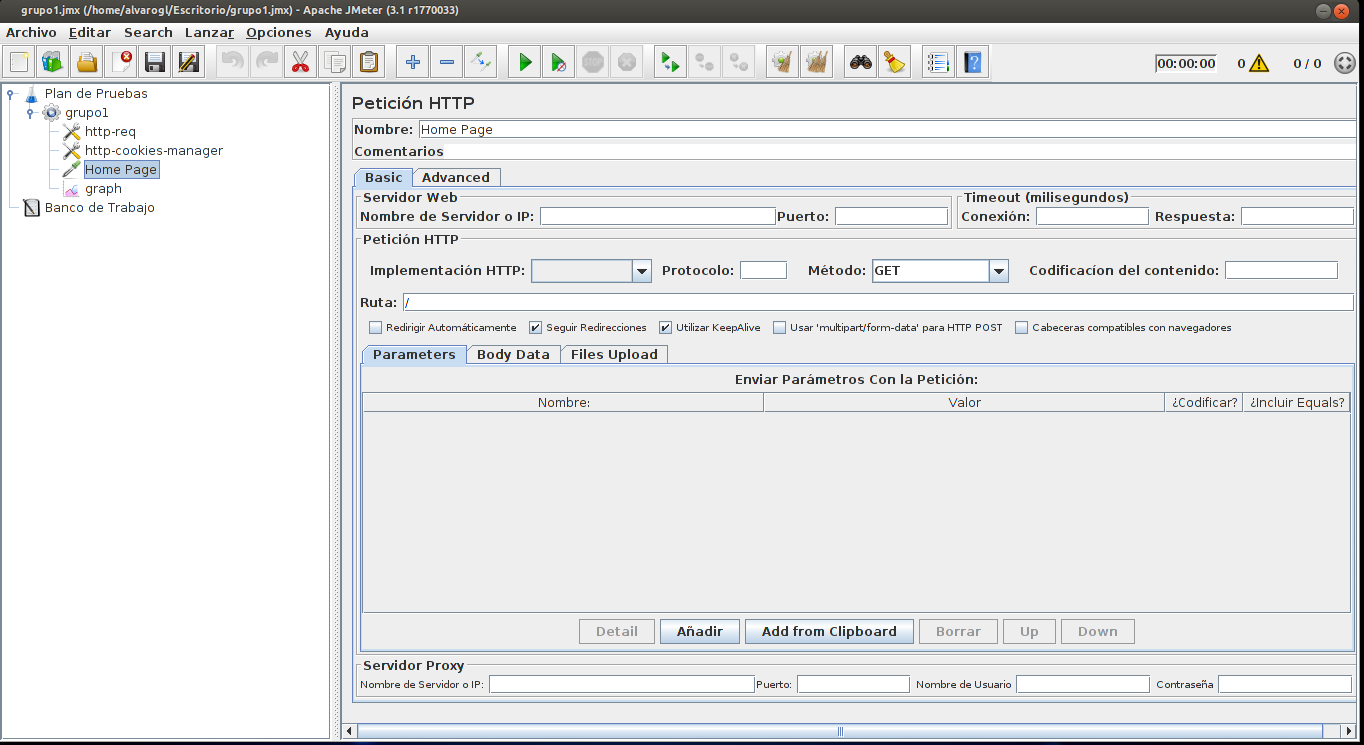
\includegraphics[scale=0.3]{cuestion4-04.png}
	\caption{Creación de las peticiones HTTP} \label{cuestion4-04}
\end{figure}

Creamos un receptor de los datos recabados en el test, en este caso, un gráfico de resultados, tal y como aparece en \ref{cuestion4-05}.

\begin{figure}[H]
	\centering
	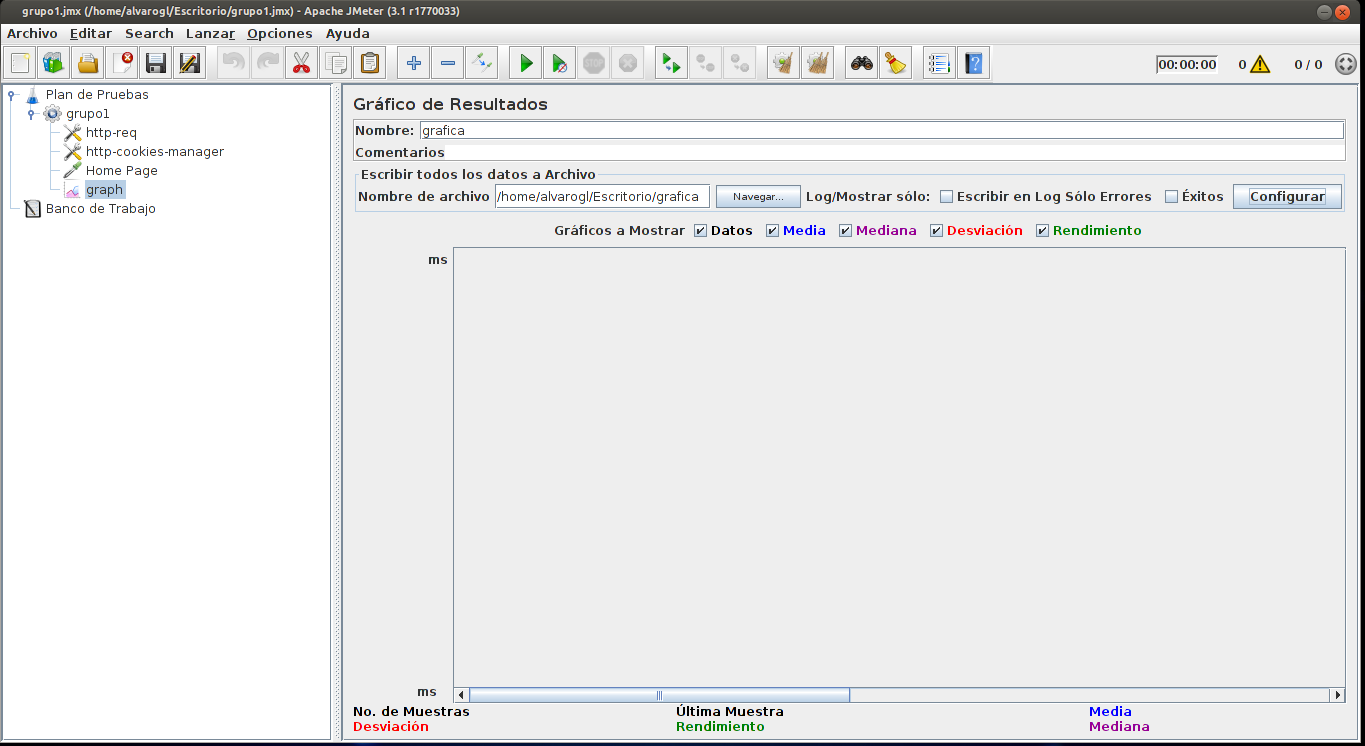
\includegraphics[scale=0.3]{cuestion4-05.png}
	\caption{Creación de un gráfico para recoger los datos} \label{cuestion4-05}
\end{figure}

Configuramos, como se ve en \ref{cuestion4-06}, el número de peticiones como en \textit{ab}, 1000 peticiones y posibilidad de ejecutar 5 simultáneamente.

\begin{figure}[H]
	\centering
	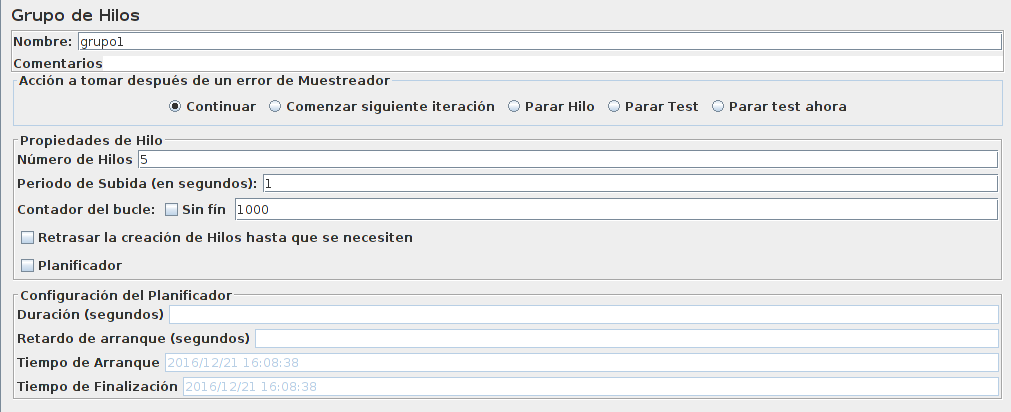
\includegraphics[scale=0.4]{cuestion4-06.png}
	\caption{Configuración del número de peticiones} \label{cuestion4-06}
\end{figure}

Los resultados del test para la máquina virtual de Ubuntu Server se muestran en \ref{cuestion4-07}.

\begin{figure}[H]
	\centering
	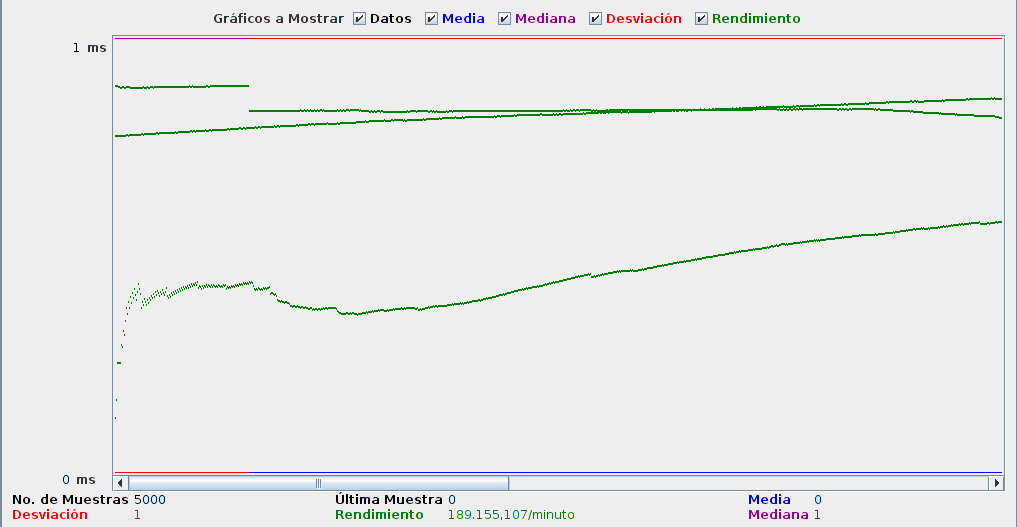
\includegraphics[scale=0.4]{cuestion4-07.png}
	\caption{Resultados del test en gráfico para Ubuntu Server} \label{cuestion4-07}
\end{figure}

El fichero de los resultados se adjuntará al archivo comprimido entregado como \url{resultados-ubuntu.csv}. En este fichero se muestran, como se observa en \ref{cuestion4-08}, algunos datos sobre la ejecución, entre ellos, el tiempo que tarda cada petición en servirse en una columna, el número de bytes por petición, el mensaje de respuesta, y la URL.

\begin{figure}[H]
	\centering
	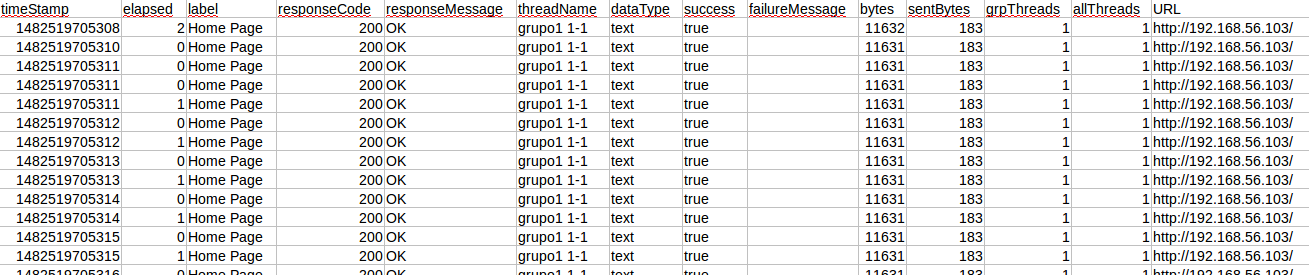
\includegraphics[scale=0.3]{cuestion4-08.png}
	\caption{Fragmento del fichero de los resultados del test (Ubuntu Server)} \label{cuestion4-08}
\end{figure}

Si realizamos la sumatoria del tiempo que tarda cada petición, y los bytes transferidos por cada una, nos salen resultados esperados, pues el número de bytes es el mismo que en la prueba realizada con \textit{ab}, aunque el tiempo transcurrido no, pero esto puede ser por el redondeo hacia arriba de los valores en la tabla. Ver \ref{cuestion4-09}.

\begin{figure}[H]
	\centering
	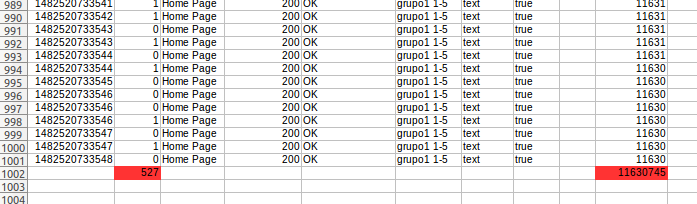
\includegraphics[scale=0.3]{cuestion4-09.png}
	\caption{Sumatoria de los datos para comprobación (Ubuntu Server)} \label{cuestion4-09}
\end{figure}

En Windows los resultados son los mostrados en \ref{cuestion4-10} y \ref{cuestion4-11}. Coinciden aproximadamente con los extraídos de \textit{ab}. El archivo adjuntado será \url{resultados-win.csv}.

\begin{figure}[H]
	\centering
	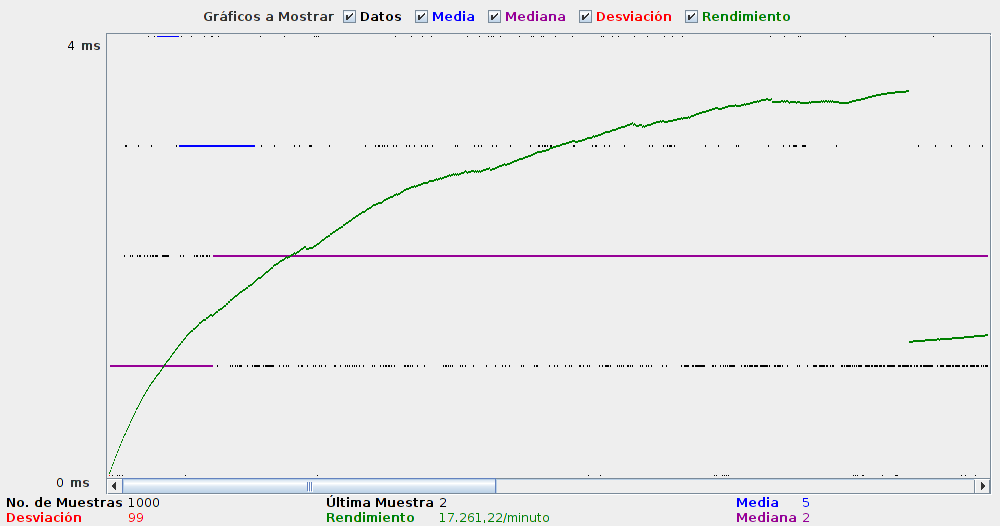
\includegraphics[scale=0.4]{cuestion4-10.png}
	\caption{Fragmento del fichero de los resultados del test (Windows)} \label{cuestion4-10}
\end{figure}

\begin{figure}[H]
	\centering
	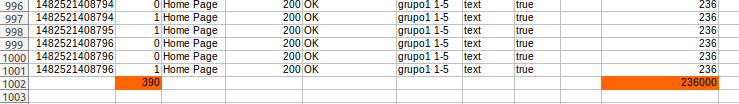
\includegraphics[scale=0.6]{cuestion4-11.png}
	\caption{Sumatoria de los datos para comprobación (Windows)} \label{cuestion4-11}
\end{figure}

Para la ejecución de CentOS ver \ref{cuestion4-12}. Los resultados se almacenarán en el archivo \url{resultados-centos.csv}

\begin{figure}[H]
	\centering
	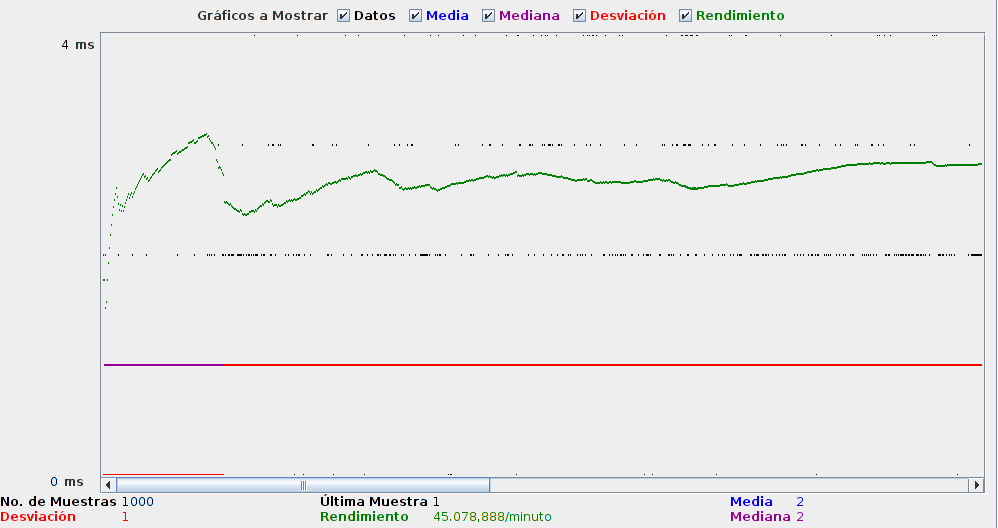
\includegraphics[scale=0.4]{cuestion4-12.png}
	\caption{Fragmento del fichero de los resultados del test (CentOS)} \label{cuestion4-12}
\end{figure}

\section{Cuestión 5. Programe un benchmark usando el lenguaje que desee. El benchmark debe incluir: \newline1) Objetivo del benchmark. \newline2) Métricas (unidades, variables, puntuaciones, etc.) \newline3) Instrucciones para su uso. \newline4) Ejemplo de uso analizando los resultados.}

\subsection{Objetivo del benchmark}

El objetivo de este \textit{benchmark} es medir el rendimiento de la CPU. Consistirá en un programa que calcule los números primos. Teniendo en cuenta que la mayoría de procesadores son de varios núcleos, la hebra principal del programa creará tantos procesos hijo (con la llamada al sistema \textit{fork}) como núcleos se indiquen en \#define NUM\_CORES.
Cada núcleo del procesador calculará números primos hasta llegar al tope indicado en \#define TOPE.
El código se adjuntará como \url{benchmark.c}

\subsection{Métricas}

Cuanto menos segundos totales tarde el procesador en calcular los primos hasta el tope, mejor rendimiento tendrá.

\subsection{Instrucciones para su uso}

\begin{itemize}
\item{Cambiar el número por defecto de \textit{núcleos} del procesador según los que tenga el mismo en \#define NUM\_CORES en el archivo \url{benchmark.c}}
\item{Ejecutar en terminal gcc -o benchmark benchmark.c}
\item{Ejecutar ./benchmark}
\end{itemize}

\subsection{Ejemplo de uso analizando los resultados}

Las pruebas serán realizadas sobre un equipo con un procesador Intel Core i7-4510U, con 2 núcleos físicos y 4 lógicos en total, a 2.60 Ghz.
En \ref{cuestion5-02} se muestra la ejecución del \textit{benchmark} sobre la máquina anfitriona con Ubuntu. Esta consigue calcular el total de números primos en 7 segundos. En \ref{cuestion5-01} se puede ver cómo efectivamente el \textit{benchmark} hace trabajar al 100\% a todos los núcleos del procesador de la máquina anfitriona, por lo que el test mide bien el rendimiento de la CPU.

\begin{figure}[H]
	\centering
	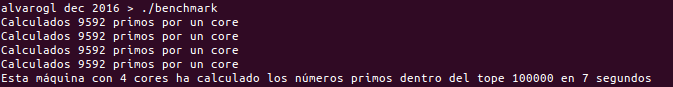
\includegraphics[scale=0.6]{cuestion5-02.png}
	\caption{Rendimiento de la CPU en máquina anfitriona de 4 núcleos} \label{cuestion5-02}
\end{figure}

\begin{figure}[H]
	\centering
	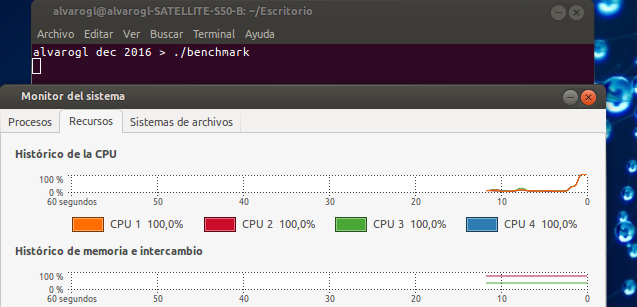
\includegraphics[scale=0.35]{cuestion5-01.png}
	\caption{Ocupación del 100\% del procesador} \label{cuestion5-01}
\end{figure}

En una máquina virtual CentOS con un solo núcleo de procesador, el resultado es de 27 segundos como se muestra en \ref{cuestion5-03}.

\begin{figure}[H]
	\centering
	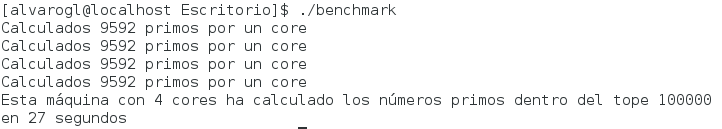
\includegraphics[scale=0.6]{cuestion5-03.png}
	\caption{Rendimiento de la CPU en máquina virtual con 1 núcleo asignado} \label{cuestion5-03}
\end{figure}

En una máquina virtual CentOS con dos núcleos asignados, la ejecución del programa tarda 10 segundos. Ver \ref{cuestion5-04}

\begin{figure}[H]
	\centering
	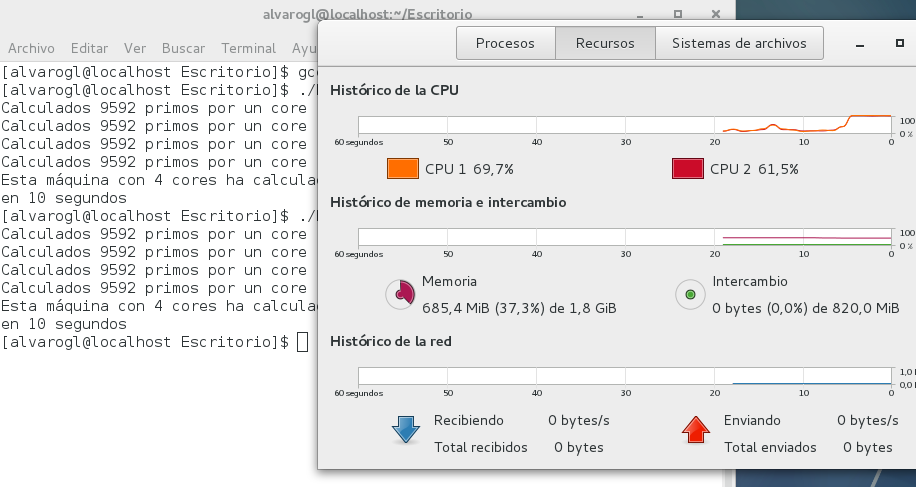
\includegraphics[scale=0.4]{cuestion5-04.png}
	\caption{Rendimiento de la CPU en máquina virtual 2 núcleos asignados} \label{cuestion5-04}
\end{figure}

También he realizado una prueba con un procesador Intel i5-4200M, con 2 núcleos físicos y 4 lógicos en total, a 2.50 Ghz, en una máquina anfitriona Fedora.
En este caso se completó la ejecución en 5 segundos, tiene un rendimiento mayor que el Intel i7-4510U. Ver \ref{cuestion5-05}.

\begin{figure}[H]
	\centering
	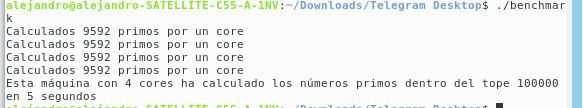
\includegraphics[scale=0.6]{cuestion5-05.png}
	\caption{Rendimiento de la CPU en máquina anfitriona con otro procesador} \label{cuestion5-05}
\end{figure}

\newpage
\bibliographystyle{plain}
\bibliography{biblio}

\end{document}